\documentclass[a4paper,14pt]{extarticle}

\usepackage[utf8x]{inputenc}
\usepackage[T1,T2A]{fontenc}
\usepackage[russian]{babel}
\usepackage{hyperref}
\usepackage{indentfirst}
\usepackage{here}
\usepackage{array}
\usepackage{graphicx}
\usepackage{caption}
\usepackage{subcaption}
\usepackage{chngcntr}
\usepackage{amsmath}
\usepackage{amssymb}
\usepackage{pgfplots}
\usepackage{pgfplotstable}
\usepackage[left=2cm,right=2cm,top=2cm,bottom=2cm,bindingoffset=0cm]{geometry}
\usepackage{multicol}

\renewcommand{\le}{\ensuremath{\leqslant}}
\renewcommand{\leq}{\ensuremath{\leqslant}}
\renewcommand{\ge}{\ensuremath{\geqslant}}
\renewcommand{\geq}{\ensuremath{\geqslant}}
\renewcommand{\epsilon}{\ensuremath{\varepsilon}}
\renewcommand{\phi}{\ensuremath{\varphi}}

\counterwithin{figure}{section}
\counterwithin{equation}{section}
\counterwithin{table}{section}
\newcommand{\sign}[1][5cm]{\makebox[#1]{\hrulefill}} % Поля подписи и даты
\graphicspath{{pics/}} % Путь до папки с картинками
\captionsetup{justification=centering,margin=1cm}
\def\arraystretch{1.3}


\begin{document}

\begin{titlepage}	% начало титульной страницы

	\begin{center}		% выравнивание по центру

		\large Санкт-Петербургский Политехнический Университет Петра Великого\\
		\large Институт компьютерных наук и технологий \\
		\large Кафедра компьютерных систем и программных технологий\\[6cm]
		% название института, затем отступ 6см
		
		\huge Метрология, стандартизация и сертификация\\[0.5cm] % название работы, затем отступ 0,5см
		\large Отчет по лабораторной работе №2\\[0.1cm]
		\large <<Регулятор мощности>>\\[6cm]

	\end{center}


	\begin{flushright} % выравнивание по правому краю
		\begin{minipage}{0.30\textwidth} % врезка в половину ширины текста
			\begin{flushleft} % выровнять её содержимое по левому краю

				\large\textbf{Работу выполнил:}\\
				\large Ламтев А.Ю.\\
				\large {Группа:} 23501/4\\
				
				\large \textbf{Преподаватель:}\\
				\large Кошелев С.И.

			\end{flushleft}
		\end{minipage}
	\end{flushright}
	
	\vfill % заполнить всё доступное ниже пространство

	\begin{center}
	\large Санкт-Петербург\\
	\large \the\year % вывести дату
	\end{center} % закончить выравнивание по центру

\thispagestyle{empty} % не нумеровать страницу
\end{titlepage} % конец титульной страницы

\vfill % заполнить всё доступное ниже пространство


%\tableofcontents
\newpage

\section{Моделирование схемы в OrCAD Capture}

\subsection{Исходная схема}

На рисунке \ref{pic:scheme} изображена схема регулятора мощности. (файл \textbf{Регулятор\_мощности.doc})

\begin{figure}[H]
\begin{center}
	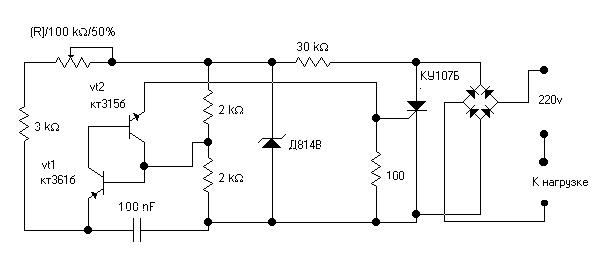
\includegraphics[width=1\textwidth]{source_schema}
	\caption{Схема регулятора мощности}
	\label{pic:scheme}
\end{center}
\end{figure}

Данная схема используется в регуляторах яркости люстры и регуляторах температуры паяльника.

На вход схемы подается напряжение $220$ В $50$ Гц. Затем через диодный мост КЦ405А ток идет на параметрический стабилизатор, образованный резистором $30$ кОм и стабилитроном Д814В. Стабилитрон Д814В служит для стабилизации и ограничения возможного повышения напряжения, питающего схему управления, а резистор $30$ кОм гасит лишнее напряжение, и напряжение опускается до напряжения стабилитрона Д814В. Дальше напряжение поступает на переменный резистор $100$ кОм и резистор $2$ кОм. Переменный резистор соединяется резистором $3$ кОм и конденсатором $100$ нФ с транзистором КТ361Б. На этой цепочке образуется задержка сигнала периодов тока, который подается на эмиттер КТ361Б. Как только на нём напряжение становится больше чем напряжение в точке соединения резисторов $2$ кОм и $2$ кОм, транзисторы открываются и весь накопленный на конденсаторе 100 нФ ток поступает на управляющий электрод тиристора, открывая его. Затем напряжение через диодный мост идет на нагрузку. Изменением сопротивления переменного резистора регулируется скорость разрядки конденсатора, от которой зависит напряжение, поступающее на нагрузку.

Свойство, оценка которого позволит судить о качестве работы -- \textbf{диапазон регулируемой мощности}.

\subsection{Элементы схемы}

В таблице \ref{tab:transistors} представлены основные параметры транзисторов \verb+КТ315Б+, \verb+BC846+, \verb+КТ361Б+ и \verb+Q2N4250+. Транзисторы \verb+КТ315Б+ и \verb+КТ361Б+ являются элементами исходной схемы, а \verb+BC846+ и \verb+Q2N4250+ соответственно их аналогами, которые есть в библиотеке \textbf{PSpice} и будут использованы при моделировании.

\begin{table}[H]
\begin{center}
	\caption{Основные параметры транзисторов}
	\label{tab:transistors}
	\def\tabcolsep{10pt}
	\begin{tabular}{|l|l|l|l|l|l|l|}
		\hline
		Наименование &
		тип & 
		$I_k$, А &
		$U_\text{кэ}$, В & 
		$P$, Вт & 
		$F$, МГц & 
		$\beta_{min}$ \\ 
		\hline
		КТ315Б &
		n-p-n &
		0.1 &
		20 &
		0.15 &
		250 &
		50 \\
		\hline
		BC846 &
		n-p-n &
		0.1 &
		65 &
		0.33 &
		250 &
		110 \\
		\hline
		КТ361Б &
		p-n-p &
		0.05 &
		20 &
		0.15 &
		250 &
		50 \\
		\hline
		Q2N4250 &
		p-n-p  &
		0.05 &
		25 &
		&
		500 &
		500 \\ 
		\hline
\end{tabular}
\end{center}
\end{table}

В таблице \ref{tab:diods} представлены основные параметры диодов \verb+КЦ405А+ и \verb+MUR160+. Диод \verb+КЦ405А+ является элементом исходной схемы, а \verb+MUR160+ - это его аналог, который есть в библиотеке \textbf{PSpice} и будет использован при моделировании.

\begin{table}[H]
\begin{center}
	\caption{Основные параметры диодов}
	\label{tab:diods}
	\def\tabcolsep{10pt}
	\begin{tabular}{|l|l|l|l|}
		\hline
		Наименование &
		$I_\text{пр max}$, А &
		$U_\text{обр}$, В &
		$U_\text{пр}$, В \\ 
		\hline
		КЦ405А &
		1 &
		600 &
		4 \\
		\hline
		MUR160 &
		1 &
		600 &
		1.35 \\
		\hline
\end{tabular}
\end{center}
\end{table}

В таблице \ref{tab:stabilitrons} представлены основные параметры стабилитронов \verb+Д814В+ (который используется в исходной схеме) и \verb+D1N758+ (аналог, который есть в библиотеке \textbf{PSpice} и будет использован при моделировании).

\begin{table}[H]
\begin{center}
	\caption{Основные параметры стабилитронов}
	\label{tab:stabilitrons}
	\def\tabcolsep{10pt}
	\begin{tabular}{|l|l|l|l|l|}
		\hline
		Наименование &
		$U_\text{ст}$, В &
		$I_\text{ст}$, мА &
		$I_\text{ст max}$, мА &
		$R_\text{дифф}$, Ом \\ 
		\hline
		Д814В &
		9---10.5 &
		3 &
		32 &
		12 \\
		\hline
		D1N758 &
		10 &
		20 &
		35 &
		17 \\
		\hline
\end{tabular}
\end{center}
\end{table}

В таблице \ref{tab:thyristors} представлены основные параметры тиристоров \verb+КУ208Г+ (который используется в исходной схеме) и \verb+MAC228A6+ (аналог, который есть в библиотеке \textbf{PSpice} и будет использован при моделировании).

\begin{table}[H]
\begin{center}
	\caption{Основные параметры тиристоров}
	\label{tab:thyristors}
	\def\tabcolsep{4pt}
	\begin{tabular}{|c|c|c|c|c|c|c|c|}
		\hline
		Наименование &
		$I_\text{пр ос}$, А &
		$U_\text{пр}$, В &
		$U_\text{вкл}$, В &
		$I_\text{зс}$, мА &
		$U_\text{отп}$, В &
		$t_\text{вкл}$, $\mu$с &
		$t_\text{выкл}$, $\mu$с \\ 
		\hline
		КУ208Г &
		5 &
		2 &
		400 &
		5 &
		5 &
		10 &
		150 \\
		\hline
		MAC228A6 &
		8 &
		2 &
		400 &
		5 &
		10 &
		1.5 &
		\\
		\hline
		%MCR729-6 &
		%5 &
		%1.5 &
		%400 &
		%10 &
		%5 &
		%0.4 &
		%15 \\
		%\hline
\end{tabular}
\end{center}
\end{table}

В таблице \ref{tab:elements_analogs} представлено соответствие элементов исходной схемы и их аналогов.

\begin{table}[H]
\begin{center}
	\caption{Активные элементы исходной схемы и их аналоги}
	\label{tab:elements_analogs}
	\def\tabcolsep{10pt}
	\begin{tabular}{|l|l|l|}
		\hline
		Класс элемента &
		Элемент исходной схемы & 
		Аналог \\
		\hline
		Транзистор &
		КТ315Б &
		BC846 \\
		\hline
		Транзистор &
		КТ361Б &
		Q2N4250 \\
		\hline
		Диод &
		КЦ405А &
		MUR160 \\
		\hline
		Стабилитрон &
		Д814В &
		D1N758 \\
		\hline
		Тиристор &
		КУ208Г &
		MAC228A6 \\
		\hline
\end{tabular}
\end{center}
\end{table}

\subsection{Схема моделирования}

Для построения схемы моделирования, изображённой на рис. \ref{pic:mod_scheme}, была создана библиотека содержащая \textbf{PSpice} модели элементов схемы, УГО которых приведено  в соответствие с ЕСКД. 

При моделировании процесса регулировки мощности устройства на вход подавалось сетевое напряжение $220$ В $50$ Гц, и на нагрузке (резистор \verb+R7+) снимались напряжение и мощность в течение $20$ миллисекунд (полный период синусоиды). Это производилось для разных значений резистора \verb+R4+ в диапазоне $0\dots100$ кОм

\begin{figure}[H]
\begin{center}
	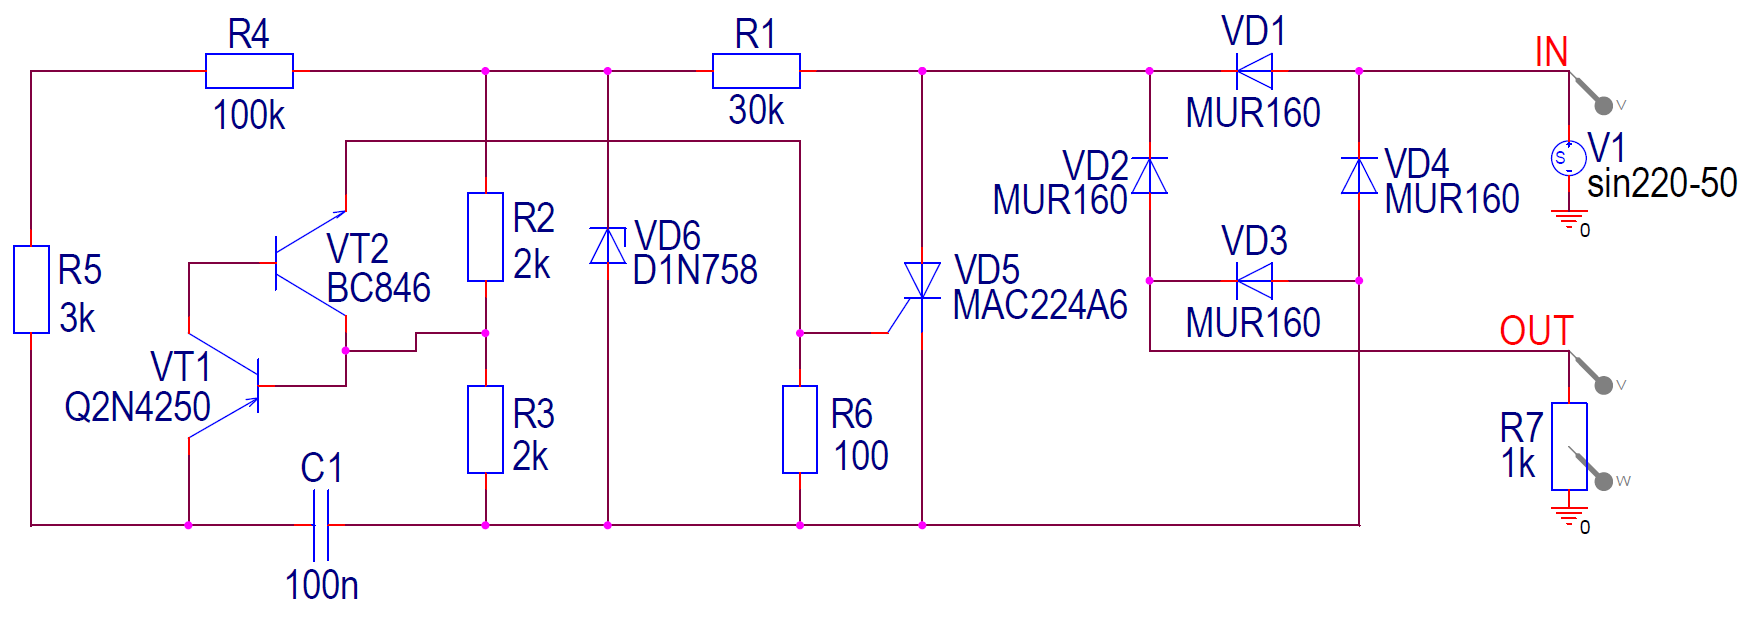
\includegraphics[width=1\textwidth]{modeling_schema}
	\caption{Схема моделирования}
	\label{pic:mod_scheme}
\end{center}
\end{figure}

\subsection{Результаты моделирования}

В результате моделирования процесса регулировки мощности устройства были построены временые диаграммы для значений переменного резистора \verb+R4+ $0$ и $100$ кОм (минимальное и максимальное значение соответственно). Они представлены на рис. \ref{pic:diag:0} -- \ref{pic:diag:100k}.

\begin{figure}[H]
\begin{center}
	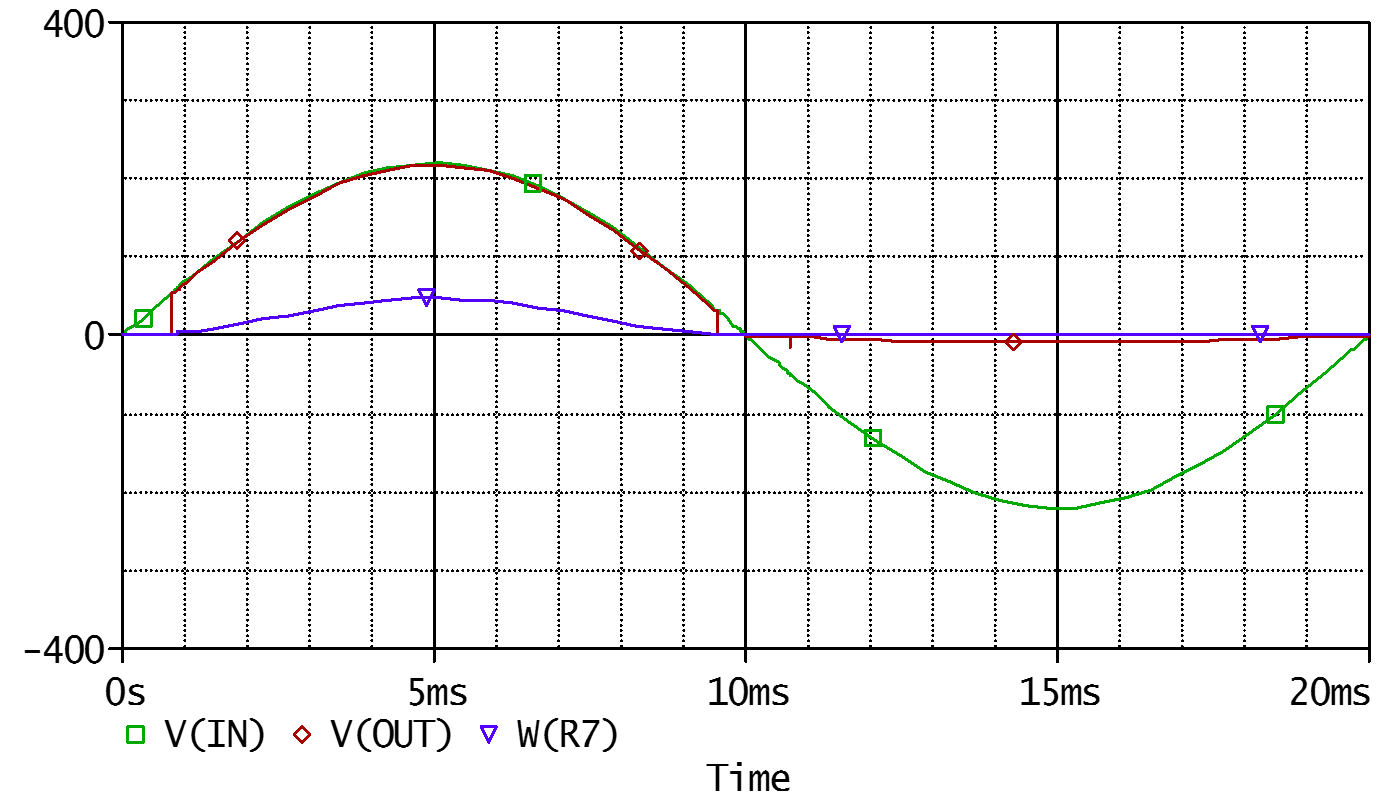
\includegraphics[width=1\textwidth]{0}
	\caption{Временная диаграмма при $R4 = 0$}
	\label{pic:diag:0}
\end{center}
\end{figure}

~

\begin{figure}[H]
\begin{center}
	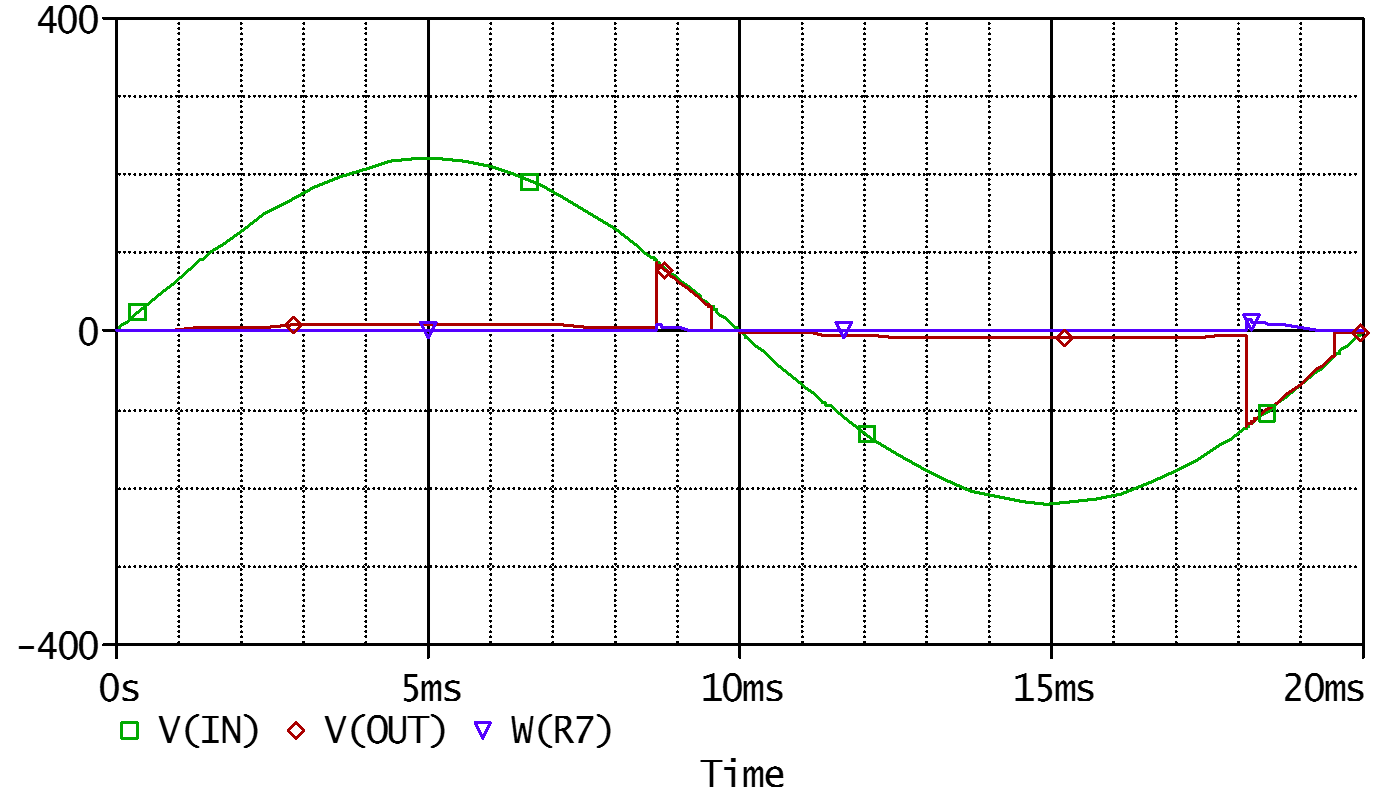
\includegraphics[width=1\textwidth]{100k}
	\caption{Временная диаграмма при $R4 = 100$ кОм}
	\label{pic:diag:100k}
\end{center}
\end{figure}

Исходя из того, что изменение значения резистора \verb+R4+ позволяет регулировать мощность на нагрузке, можно сделать вывод о правильной работе схемы.

\subsection{Измеряемые величины}

Измерение диапазона регулируемой мощности позволит оценить работу устройства количественно.

Будем считать границы диапазона регулируемой мощности как отношение площадей под графиками -- полученной при граничном значении резистора \verb+R4+ к идеальной:

\begin{equation}
\label{eq:d:i}
	d_i = \frac{\int_{t_{i1}}^{t_{i2}} P(t) dt}{\int_{0}^{10} P(t) dt} \cdot 100\% \text{, i = 1,2}
\end{equation}

\begin{equation}
	D = [d_1, d_2]
\end{equation}

Синусоидальное напряжение описывается уравнением \ref{eq:u:gen}: 

\begin{equation}
\label{eq:u:gen}
	U(t) = U_m \cdot sin(\omega t + \phi)
\end{equation}

\noindent где $U_m = 220$ В -- амплитуда, $\omega = 2 \pi f = 100 \pi$ -- циклическая частота, $\phi = 0$ -- начальная фаза. Получаем уравнение \ref{eq:u:der}:

\begin{equation}
\label{eq:u:der}
	U(t) = 220 \cdot sin \left(100 \pi t \right)
\end{equation}

Мощность описывается уравнением \ref{eq:p}:

\begin{equation}
\label{eq:p}
	P(t) = \frac{48400}{R} \cdot sin^2 \left(100 \pi t \right)
\end{equation}

Вычислим площадь под графиком мощности для полного полупериода синусоиды:

\begin{displaymath}
	S = \int_{0}^{10} P(t) dt = \int_{0}^{10} \frac{48400}{R} \cdot sin^2 \left(100 \pi t \right) dt = \frac{242000}{R}
\end{displaymath}

Для определения границ диапазона необходимо определить моменты времени, в которые \verb+VD5+ включается и выключается, для значений \verb+R4+ = $0$ и $100$ кОм.

\begin{itemize}

	\item $R4 = 100$ кОм
	
		Для положительного полупериода момент включения тиристора $t_{11} \approx 8.7$ мс, момент выключения тиристора $t_{12} \approx 9.8$ мс. Для отрицательного полупериода -- $t_{11} \approx 8.2$ мс и $t_{12} \approx 9.8$ мс. $\overline{{t_{11}}} \approx 8.45$\\
		
		\begin{displaymath}
			d_1 = \frac{\int_{t_{11}}^{t_{12}} P(t) dt}{\int_{0}^{10} P(t) dt} \cdot 100\% = \frac{\int_{8.45}^{9.8} \frac{48400}{R} \cdot sin^2 \left(100 \pi t \right)}{\frac{242000}{R}} \cdot 100\% = \frac{\frac{32670}{R}}{\frac{242000}{R}} \cdot 100\% = \frac{32670}{242000} \cdot 100\% = 13.5 \%
		\end{displaymath}		
		
	\item $R4 = 0$
	
		Для положительного полупериода момент включения тиристора $t_{21} \approx 0.8$ мс, момент выключения тиристора $t_{22} \approx 9.8$ мс. Для отрицательного полупериода -- $t_{21} \approx 0.8$ мс и $t_{22} \approx 9.8$ мс.\\
		Вычислим границу диапазона по формуле \ref{eq:d:i}:
		
		\begin{displaymath}
			d_2 = \frac{\int_{t_{21}}^{t_{22}} P(t) dt}{\int_{0}^{10} P(t) dt} \cdot 100\% = \frac{\int_{0.8}^{9.8} \frac{48400}{R} \cdot sin^2 \left(100 \pi t \right)}{\frac{242000}{R}} \cdot 100\% = \frac{\frac{217800}{R}}{\frac{242000}{R}} \cdot 100\% = \frac{217800}{242000} \cdot 100\% = 90 \%
		\end{displaymath}
		
\end{itemize}

\begin{displaymath}
	D = [13.5\% , 90\% ]
\end{displaymath}

\section{Оценка априорной инструментальной погрешности измерений}

\subsection{Методы измерений}

Чтобы оценить диапазон регулируемой мощности, необходимо для минимального и максимального значения переменного резистора \verb+R4+ ($0$ Ом и $100$ кОм соответственно) подключить к нагрузке осциллограф и при помощи курсоров измерить моменты времени включения и выключения тиристора \verb+VD5+.

\subsection{Средства измерений}

Необходимые измерения можно выполнить, воспользовавшись цифровым осциллографом \verb+Актаком ADS-2061M+, который есть в лаборатории электроники и электротехники кафедры. Абсолютная погрешность курсорных измерений временного интервала этого осциллографа вычисляется по формуле \ref{eq:2:1}:

\begin{equation}
\label{eq:2:1}
	\Delta t = \pm \left(0.02 \cdot t_{\text{и}} + 0.04 \cdot K_{\text{р}} \right)
\end{equation}

\noindent где $t_{\text{и}}$ -- измеренное значение временного интервала, $K_{\text{р}}$ -- установленное значение коэффициента развертки. $K_{\text{р}}$ $\in$ $\left[5 \frac{\text{нс}}{\text{дел}} , 100 \frac{\text{с}}{\text{дел}}\right]$, шаг $1$-$2$-$5$.

\subsection{Погрешность измерений}

Согласно формуле \ref{eq:2:1} измеренные значения $t_{11}$, $t_{12}$, $t_{21}$ и $t_{22}$ имеют погрешность аддитивно-мультипликативного характера. Необходимо выбрать коэффициент $K_{\text{р}}$ таким образом, чтобы моменты времени включения и выключения тиристора \verb+VD5+ занимали большую часть дисплея осциллографа. Осциллограф имеет 15 горизонтальных делений. Следовательно значение $K_{\text{р}}$ должно быть наименьшим из удовлетворяющих условию $K_{\text{р}} \geq \frac{t_{\text{и}}}{15}$. Поэтому для полученного в результате моделирования значения $t_{11} \approx 0.8$ мс $K_{\text{р}} = 0.054$, для $t_{12} = t_{22} \approx 9.8$ мс $K_{\text{р}} = 0.654$, для $t_{21} \approx 8.45$ мс $K_{\text{р}} = 0.564$.
Таким образом, абсолютные погрешности у полученных в результате моделирования значений будут следующими:

\begin{displaymath}
	\Delta t_{11} = \pm \left( 0.02 \cdot t_{11} + 0.04 \cdot K_{\text{р}} \right) \text{ мс} = \pm \left( 0.02 \cdot 0.8 + 0.04 \cdot 0.054 \right) \text{ мс} = \pm 0.01816 \text{ мс} 
\end{displaymath}

\begin{displaymath}
	\Delta t_{12} = \Delta t_{22} = \pm \left( 0.02 \cdot t_{12} + 0.04 \cdot K_{\text{р}} \right) \text{ мс} = \pm \left( 0.02 \cdot 9.8 + 0.04 \cdot 0.654 \right) \text{ мс} = \pm 0.22216 \text{ мс}
\end{displaymath}

\begin{displaymath}
	\Delta t_{21} = \pm \left( 0.02 \cdot t_{21} + 0.04 \cdot K_{\text{р}} \right) \text{ мс} = \pm \left( 0.02 \cdot 8.45 + 0.04 \cdot 0.564 \right) \text{ мс} = \pm 0.19156 \text{ мс}
\end{displaymath}

Относительная погрешность измеряемой величины вычисляется по формуле:

\begin{equation}
	\delta x = \frac{\Delta x}{x} \cdot 100\%
\end{equation}

Поэтому относительные погрешности у полученных в результате моделирования значений будут следующими:

\begin{displaymath}
	\delta t_{11} = \frac{\Delta t_{11}}{t_{11}} \cdot 100\% = \frac{0.01816 \text{ мс}}{0.8 \text{ мс}} \cdot 100\% \approx 2.27 \%
\end{displaymath}

\begin{displaymath}
	\delta t_{12} = \delta t_{22} = \frac{\Delta t_{12}}{t_{12}} \cdot 100\% = \frac{0.22216 \text{ мс}}{9.8 \text{ мс}} \cdot 100\% \approx 2.27 \%
\end{displaymath}

\begin{displaymath}
	\delta t_{21} = \frac{\Delta t_{21}}{t_{21}} \cdot 100\% = \frac{0.19156 \text{ мс}}{8.45 \text{ мс}} \cdot 100\% \approx 2.27 \%
\end{displaymath}

Границы диапазона регулирования мощности вычисляются по формуле\\\noindent $d_i = \frac{\int_{t_{i1}}^{t_{i2}} P(t) dt}{\int_{0}^{10} P(t) dt} \cdot 100\% \text{, i = 1,2}$, и измеренные величины некоррелированные, поэтому:

\begin{displaymath}
\begin{aligned}
	\delta d_1 = \sqrt{(\delta t_{11})^2 + (\delta t_{12})^2} = \sqrt{(2.27\%)^2 + (2.27\%)^2} = 3.21 \%
\end{aligned}
\end{displaymath}

\begin{displaymath}
\begin{aligned}
	\delta d_2 = \sqrt{(\delta t_{21})^2 + (\delta t_{22})^2} = \sqrt{(2.27\%)^2 + (2.27\%)^2} = 3.21 \%
\end{aligned}
\end{displaymath}

Абсолютная погрешность измеряемой величины вычисляется по формуле:

\begin{equation}
	\Delta x = \frac{x \cdot \delta x}{100 \%}
\end{equation}

Поэтому абсолютные погрешности границ диапазона регулирования мощности равны:

\begin{displaymath}
	\Delta d_1 = \frac{d_1 \cdot \delta d_1}{100 \%} = \frac{13.5 \% \cdot 3.21 \%}{100 \%} \approx 0.43 \%
\end{displaymath}

\begin{displaymath}
	\Delta d_2 = \frac{d_2 \cdot \delta d_2}{100 \%} = \frac{90 \% \cdot 3.21 \%}{100 \%} \approx 2.89 \%
\end{displaymath}

\begin{displaymath}
	d_1 = (13.5 \pm 0.4)\%
\end{displaymath}

\begin{displaymath}
	d_2 = (90.0 \pm 2.9)\%
\end{displaymath}

\end{document}
